\section{Actividad No 02 – Adicionar Gráficos al Reporte} 

\begin{enumerate}[1.]
	\item Arrastrar el campo SalesYTD a la casilla Valores (Values). El gráfico se llenará con datos.
	\\
	\\

	\begin{center}
	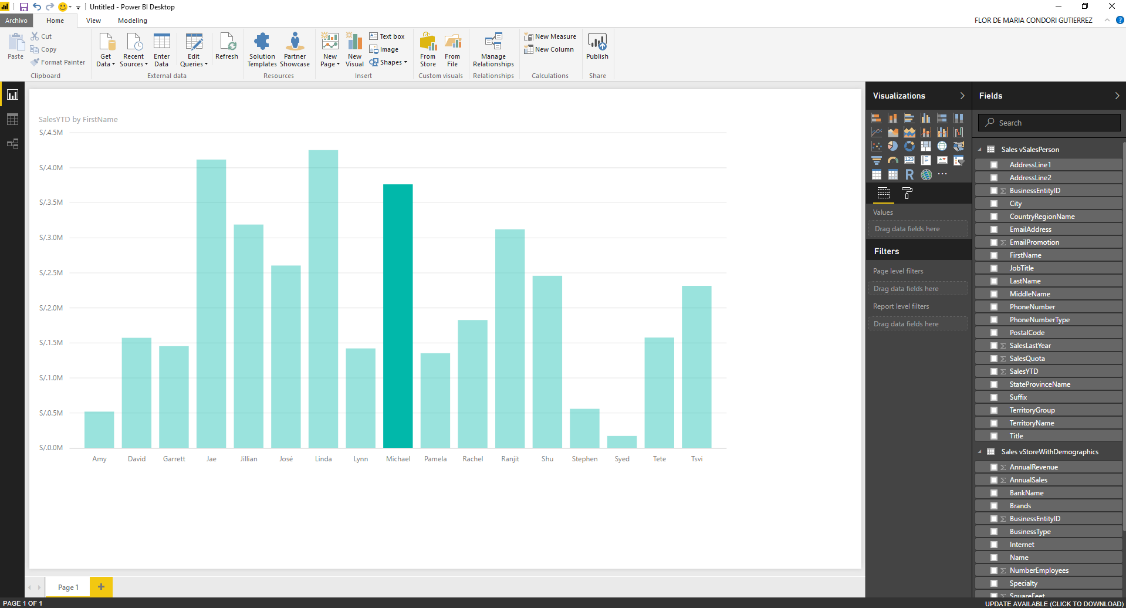
\includegraphics[width=16cm]{./Imagenes/21} 
	\end{center}

	\item Cambiar el color para Jae, Linda, y Michael a rojo.
	\\
	\\

	\begin{center}
	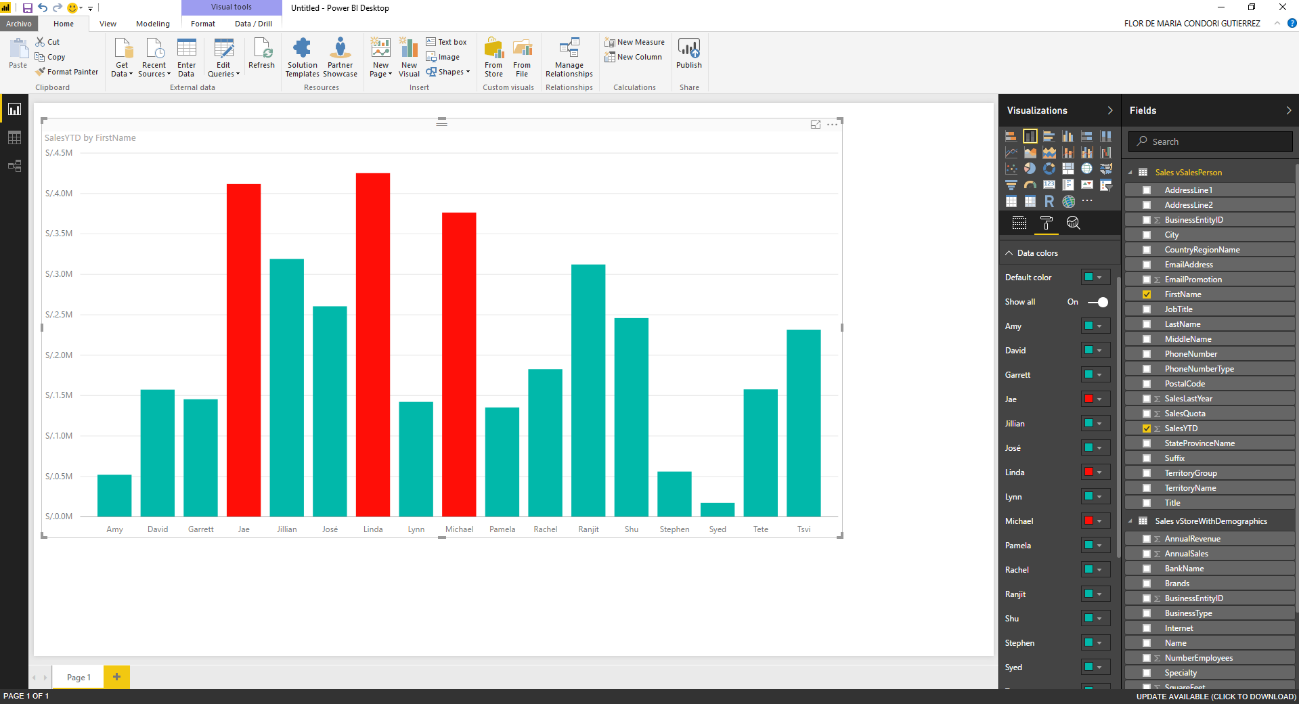
\includegraphics[width=16cm]{./Imagenes/22} 
	\end{center}

	\item En el panel Campos, hacer click en la elipsis (…) contigua a AnnualRevenue, y hacer click en Renombrar (Rename). Tipear Beneficios anuales luego presionar Enter.
	\\
\\
	
	\begin{center}
	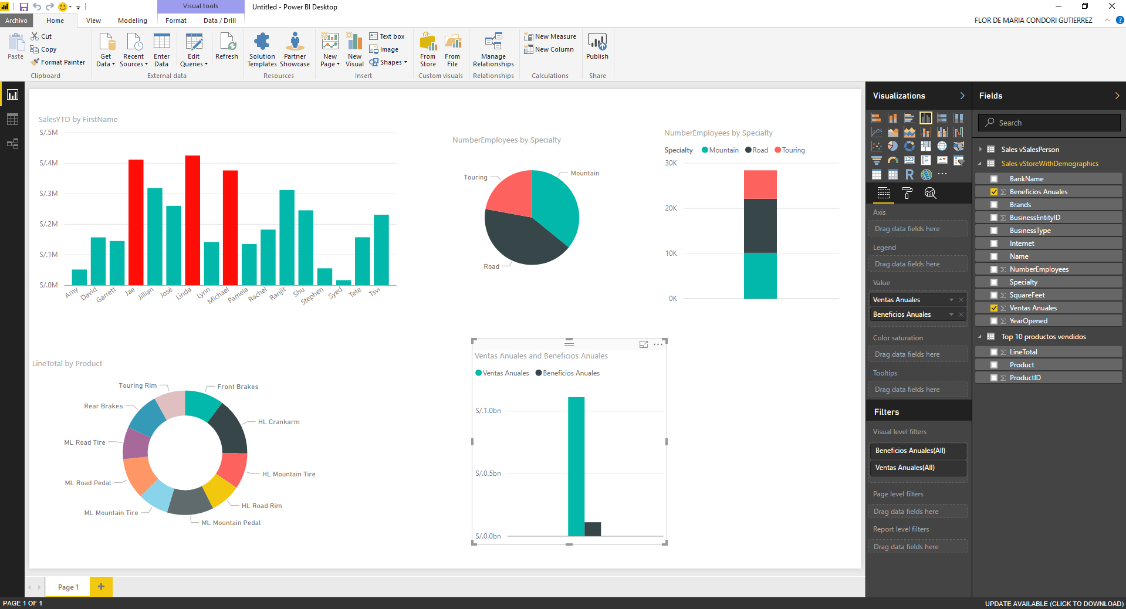
\includegraphics[width=16cm]{./Imagenes/23} 
	\end{center}


	\item Expandir la Información de página (Page Information), y en la casilla Nombre tipear Ventas. Hacer click en el área de reporte y apreciar que el nombre ha cambiado en la pestaña al final del reporte.
	\\
	\\
	\begin{center}
	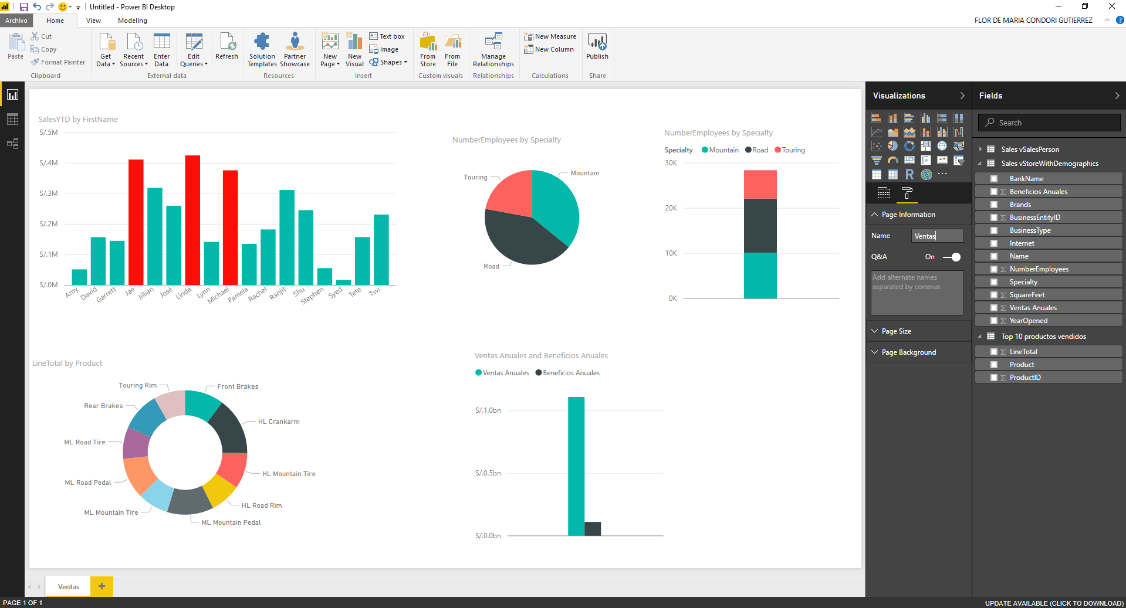
\includegraphics[width=16cm]{./Imagenes/24} 
	\end{center}

	\item En el menu Archivo (File menu), hacer click en Guardar (Save), crear un directorio Power BI, y guardar el archive como Ventas de Adventure Works Sales.
	\\
	\\
	\begin{center}
	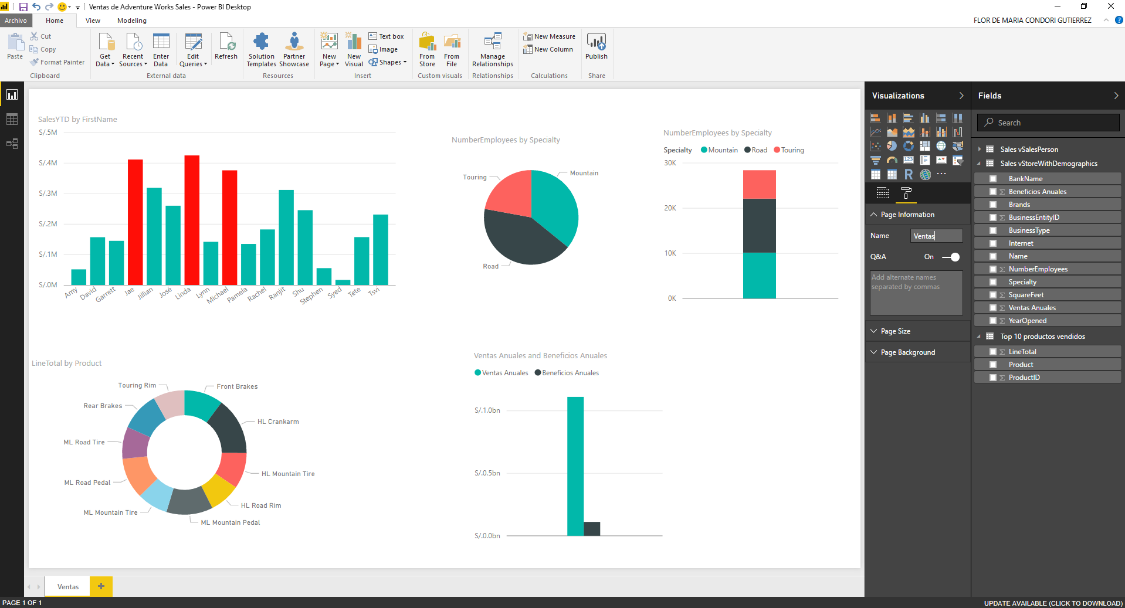
\includegraphics[width=16cm]{./Imagenes/25} 
	\end{center}

\end{enumerate}


